% Provenance (never printed): cycle 3 "La planete Terre. Les etres vivants
% dans leur environnement" (natural phenomena: volcanoes and earthquakes,
% natural hazards and the behaviour to adopt); see sources/book1/PROVENANCE.md.
% Book 1, grade 4, chapter 2.
\chapter{Volcans et séismes~: un premier regard}\label{ch:g4:volcanoes-earthquakes-first-look}

Lundi soir, les informations montrent un \omterm{def:g4:volcanoes-earthquakes-first-look:volcano}{volcan} sur une île lointaine. Dans
la nuit, une fontaine de \omterm{def:g3:stones-pebbles-sand:rock}{roche} orange incandescente jaillit d'une fissure
du sol, et des \omterm{def:g1:landscapes-around-us:water}{rivières} de feu descendent lentement la pente jusqu'à la
\omterm{def:g2:water-on-earth:ocean}{mer}, en sifflant et en fumant. Jeudi, les informations montrent un autre
endroit~: une petite ville où, à l'aube, le sol a tremblé pendant une
demi-minute. Des cheminées sont tombées dans la rue, et une vieille maison
a glissé de ses fondations.

Deux événements très différents. Pourtant, tous deux viennent des
profondeurs de la Terre et, nous allons le voir, tous deux se produisent
bien plus souvent dans certaines régions du monde que dans d'autres.

\begin{recall}
Les \omterm{def:g1:landscapes-around-us:landform}{montagnes}, les \omterm{def:g1:landscapes-around-us:landform}{collines}, les \omterm{def:g1:landscapes-around-us:landform}{vallées} et les \omterm{def:g1:landscapes-around-us:landform}{plaines} sont les formes du
relief (\cref{ch:g1:landscapes-around-us}). Les terres de la Terre sont
rassemblées en sept \omterm{def:g3:continents-and-oceans:continent}{continents}, entre cinq \omterm{def:g2:water-on-earth:ocean}{océans}~; le Pacifique est le
plus grand \omterm{def:g2:water-on-earth:ocean}{océan} (\cref{ch:g3:continents-and-oceans}).
\end{recall}

\section{Un volcan entre en éruption}

Loin sous nos pieds, la Terre est très chaude. À certains endroits, la
\omterm{def:g3:stones-pebbles-sand:rock}{roche} y est si chaude qu'elle a fondu. Cette \omterm{def:g3:stones-pebbles-sand:rock}{roche} fondue est plus légère
que la \omterm{def:g3:stones-pebbles-sand:rock}{roche} solide qui l'entoure~: elle monte donc lentement, comme un
bouchon dans l'eau. Là où elle trouve un chemin jusqu'à la surface, un
\omterm{def:g4:volcanoes-earthquakes-first-look:volcano}{volcan} naît.

\begin{definition}[Volcan]\label{def:g4:volcanoes-earthquakes-first-look:volcano}
Un \emph{volcan}\index{volcan} est un endroit où de la \omterm{def:g3:stones-pebbles-sand:rock}{roche} fondue venue
des profondeurs de la Terre sort à la surface, ainsi que la \omterm{def:g1:landscapes-around-us:landform}{colline} ou la
\omterm{def:g1:landscapes-around-us:landform}{montagne} que la \omterm{def:g3:stones-pebbles-sand:rock}{roche} fondue y construit, couche après couche.
\end{definition}

\begin{definition}[Éruption, lave et cendres volcaniques]\label{def:g4:volcanoes-earthquakes-first-look:eruption}
Une \emph{éruption}\index{eruption@éruption} est le moment où un \omterm{def:g4:volcanoes-earthquakes-first-look:volcano}{volcan}
rejette de la \omterm{def:g3:stones-pebbles-sand:rock}{roche} fondue, des cendres et des gaz. La \emph{lave}\index{lave}
est de la \omterm{def:g3:stones-pebbles-sand:rock}{roche} fondue qui se répand à la surface~; elle coule, puis se
refroidit et durcit en une \omterm{def:g3:stones-pebbles-sand:rock}{roche} nouvelle. Les
\emph{cendres volcaniques}\index{cendres volcaniques} sont faites de
minuscules morceaux de \omterm{def:g3:stones-pebbles-sand:rock}{roche} et de verre projetés dans l'air par une
éruption~; elles retombent comme une \omterm{def:g4:clouds-rain-snow:precipitation}{neige} grise.
\end{definition}

\begin{omfigure}
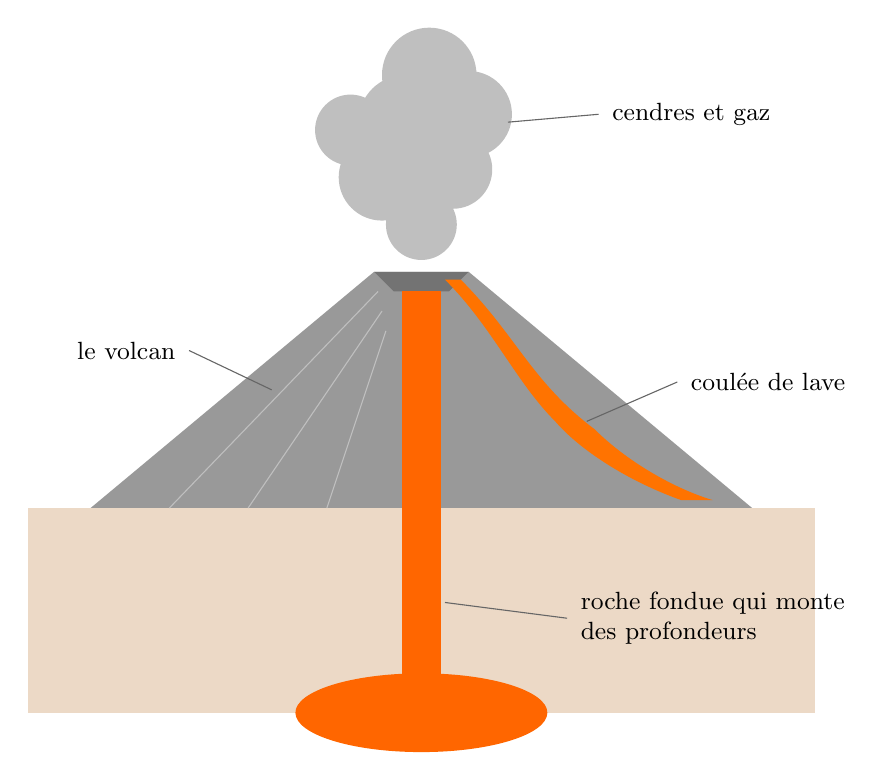
\begin{tikzpicture}[font=\small]
  % ground and deep rock
  \fill[brown!30] (-5,-2.6) rectangle (5,0);
  % the volcano
  \fill[black!40] (-4.2,0) -- (-0.6,3.0) -- (0.6,3.0) -- (4.2,0) -- cycle;
  \fill[black!55] (-0.6,3.0) -- (-0.35,2.75) -- (0.35,2.75) -- (0.6,3.0) -- cycle;
  % layers inside the cone
  \foreach \k in {1,2,3}
    \draw[black!25] (-4.2+1.0*\k,0) -- (-0.6+0.05*\k,3.0-0.25*\k);
  % molten rock rising from deep below
  \fill[orange!80!red] (-0.25,-2.6) -- (-0.25,2.75) -- (0.25,2.75) -- (0.25,-2.6) -- cycle;
  \fill[orange!80!red] (0,-2.6) ellipse (1.6 and 0.5);
  % lava flow on the right flank
  \fill[orange!90!red] (0.5,2.9) .. controls (1.2,2.2) and (1.4,1.6) .. (2.2,1.0)
    .. controls (2.6,0.6) and (3.2,0.25) .. (3.7,0.1) -- (3.3,0.1)
    .. controls (2.6,0.35) and (2.0,0.75) .. (1.7,1.1)
    .. controls (1.2,1.6) and (0.9,2.3) .. (0.3,2.9) -- cycle;
  % ash and gas cloud
  \foreach \x/\y/\r in {0/3.6/0.45, -0.5/4.2/0.55, 0.4/4.3/0.5, -0.2/4.9/0.6, 0.6/5.0/0.55, -0.9/4.8/0.45, 0.1/5.5/0.6}
    \fill[black!25] (\x,\y) circle (\r);
  % labels
  \node[anchor=west] at (2.3,5.0) {cendres et gaz};
  \draw[black!60] (2.25,5.0) -- (1.1,4.9);
  \node[anchor=west] at (3.3,1.6) {coulée de lave};
  \draw[black!60] (3.25,1.6) -- (2.1,1.1);
  \node[anchor=east] at (-3.0,2.0) {le volcan};
  \draw[black!60] (-2.95,2.0) -- (-1.9,1.5);
  \node[anchor=west, align=left] at (1.9,-1.4) {roche fondue qui monte\\des profondeurs};
  \draw[black!60] (1.85,-1.4) -- (0.3,-1.2);
\end{tikzpicture}

{\small Un \omterm{def:g4:volcanoes-earthquakes-first-look:volcano}{volcan} en \omterm{def:g4:volcanoes-earthquakes-first-look:eruption}{éruption} (dessin, sans respect de l'échelle). La \omterm{def:g3:stones-pebbles-sand:rock}{roche}
fondue monte des profondeurs et sort au sommet~: elle descend en coulées
de \omterm{def:g4:volcanoes-earthquakes-first-look:eruption}{lave}, tandis que les cendres et les gaz sont projetés vers le ciel.
Chaque \omterm{def:g4:volcanoes-earthquakes-first-look:eruption}{éruption} ajoute une nouvelle couche à la \omterm{def:g1:landscapes-around-us:landform}{montagne}.}
\label{fig:g4:volcanoes-earthquakes-first-look:volcano}
\end{omfigure}

Les \omterm{def:g4:volcanoes-earthquakes-first-look:eruption}{éruptions} ne se ressemblent pas toutes. Dans certaines, la \omterm{def:g4:volcanoes-earthquakes-first-look:eruption}{lave} est
fluide~: elle s'écoule tranquillement en \omterm{def:g1:landscapes-around-us:water}{rivières} incandescentes qui
peuvent couler sur des kilomètres, parfois jusqu'à la \omterm{def:g2:water-on-earth:ocean}{mer}. Dans d'autres,
la \omterm{def:g3:stones-pebbles-sand:rock}{roche} fondue est épaisse et pleine de gaz, comme une bouteille de
boisson gazeuse qu'on a secouée~: quand elle jaillit, elle explose en une
immense colonne de cendres qui monte très haut dans le ciel.

\begin{omfigure}
\begin{minipage}[b]{0.56\linewidth}\centering
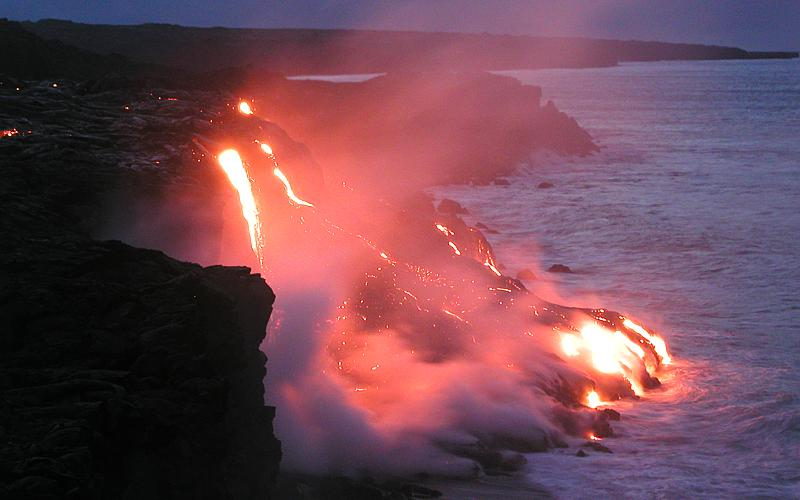
\includegraphics[width=\linewidth]{images/book1/g4-lava-ocean.jpg}

{\small Une \omterm{def:g4:volcanoes-earthquakes-first-look:eruption}{éruption} à \omterm{def:g4:volcanoes-earthquakes-first-look:eruption}{lave} fluide~: la \omterm{def:g4:volcanoes-earthquakes-first-look:eruption}{lave} coule le long d'une falaise
jusque dans l'\omterm{def:g2:water-on-earth:ocean}{océan}, à Hawaï. Photographie~: USGS Hawaiian Volcano
Observatory (domaine public).}
\end{minipage}\hfill
\begin{minipage}[b]{0.4\linewidth}\centering
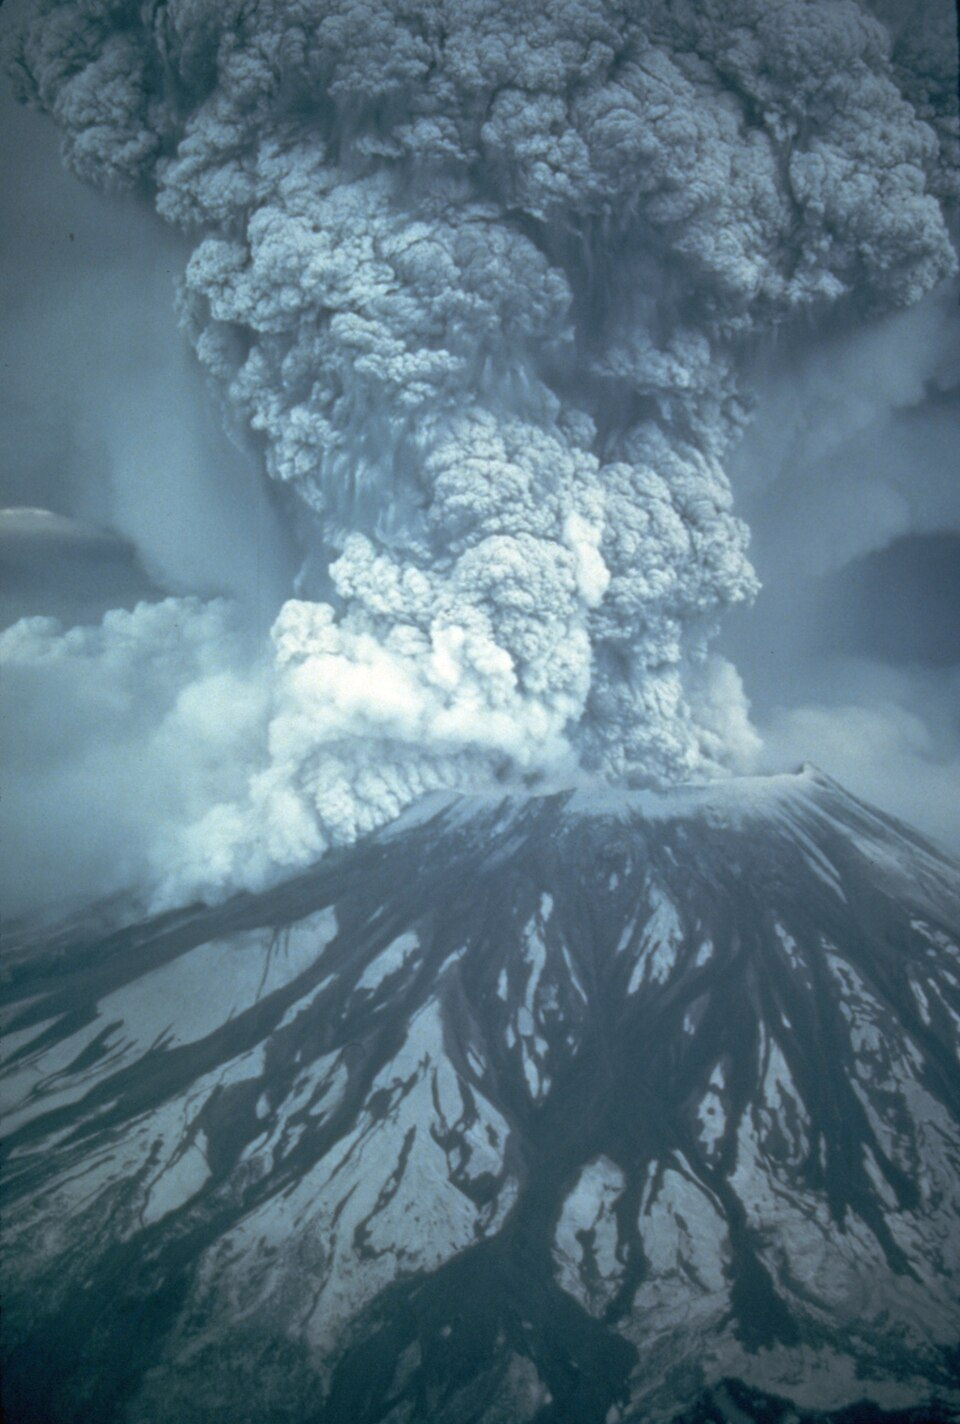
\includegraphics[width=0.78\linewidth]{images/book1/g4-st-helens.jpg}

{\small Une \omterm{def:g4:volcanoes-earthquakes-first-look:eruption}{éruption} explosive~: le mont Saint Helens, aux États-Unis, le
18~mai 1980. Photographie~: Austin Post, USGS (domaine public).}
\end{minipage}
% ledger: usgs:pu-oo-ocean, usgs:msh-1980
\label{fig:g4:volcanoes-earthquakes-first-look:two-eruptions}
\end{omfigure}

\begin{example}[Le mont Saint Helens, 1980]\label{ex:g4:volcanoes-earthquakes-first-look:st-helens}
Au printemps 1980, un renflement a grossi sur le flanc du mont Saint
Helens, poussé par la \omterm{def:g3:stones-pebbles-sand:rock}{roche} fondue qui montait à l'intérieur de la
\omterm{def:g1:landscapes-around-us:landform}{montagne}. Le matin du 18~mai, un petit \omterm{def:g4:volcanoes-earthquakes-first-look:earthquake}{séisme} a secoué la \omterm{def:g1:landscapes-around-us:landform}{montagne}, le
renflement s'est effondré en un gigantesque glissement de terrain, et le
\omterm{def:g4:volcanoes-earthquakes-first-look:volcano}{volcan} a explosé vers le côté et vers le haut. Les 400~mètres du sommet de
la \omterm{def:g1:landscapes-around-us:landform}{montagne} avaient disparu~: le sommet était devenu un immense cratère.
% ledger: usgs:msh-1980
\end{example}

\section{Le sol tremble}

Les \omterm{def:g3:stones-pebbles-sand:rock}{roches} loin sous nos pieds ne sont pas parfaitement immobiles. Très
lentement, elles sont poussées et tirées. Elles se plient un peu, comme
une règle que l'on pousse par les deux bouts --- jusqu'à ce que,
brusquement, elles se cassent et glissent. La secousse fait trembler le sol
sur des kilomètres à la ronde.

\begin{definition}[Séisme]\label{def:g4:volcanoes-earthquakes-first-look:earthquake}
Un \emph{séisme}\index{seisme@séisme}, ou tremblement de terre, est une
secousse brutale du sol, causée par des \omterm{def:g3:stones-pebbles-sand:rock}{roches} qui se cassent et glissent
en profondeur.
\end{definition}

Un \omterm{def:g4:volcanoes-earthquakes-first-look:earthquake}{séisme} ne dure en général que quelques secondes, parfois une minute ou
deux pour les plus forts. La plupart des \omterm{def:g4:volcanoes-earthquakes-first-look:earthquake}{séismes} sont si faibles que
personne ne les sent~: seuls des instruments les remarquent. Un \omterm{def:g4:volcanoes-earthquakes-first-look:earthquake}{séisme}
fort peut faire onduler le sol comme le pont d'un bateau, fissurer les
routes et faire tomber des murs et des maisons.

\begin{omfigure}
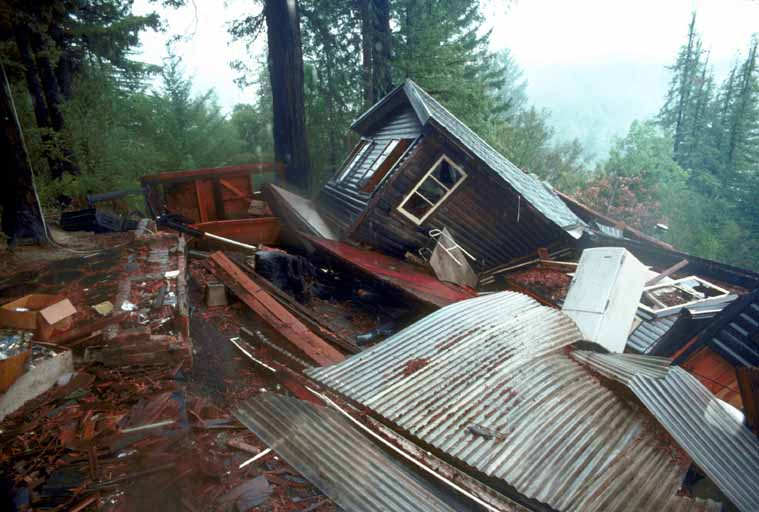
\includegraphics[width=0.55\linewidth]{images/book1/g4-loma-prieta-house.jpg}

{\small Après un fort \omterm{def:g4:volcanoes-earthquakes-first-look:earthquake}{séisme} en Californie, en 1989~: cette maison en bois
a été projetée sur le côté, hors de ses fondations en béton.
Photographie~: J.~K.~Nakata, USGS (domaine public).}
% ledger: usgs:loma-prieta-house
\end{omfigure}

\begin{remark}[À quelle fréquence~?]\label{rem:g4:volcanoes-earthquakes-first-look:how-often}
Les géologues tiennent la liste de tous les grands \omterm{def:g4:volcanoes-earthquakes-first-look:earthquake}{séismes} de la Terre. Sur
les 50 années de 1976 à 2025, cette liste compte 7\,031 grands \omterm{def:g4:volcanoes-earthquakes-first-look:earthquake}{séismes}
(assez forts pour endommager les bâtiments proches)~: environ 141 par an,
soit presque 3 chaque semaine. Les plus forts de tous, qui peuvent détruire
des villes entières, sont environ 14 par an. Sur la même Terre, environ
1\,200 \omterm{def:g4:volcanoes-earthquakes-first-look:volcano}{volcans} sont entrés en \omterm{def:g4:volcanoes-earthquakes-first-look:eruption}{éruption} depuis une douzaine de milliers
d'années.
% ledger: data:usgs-comcat, data:gvp
\end{remark}

\section{Où se produisent les volcans et les séismes}

Si les \omterm{def:g4:volcanoes-earthquakes-first-look:volcano}{volcans} et les \omterm{def:g4:volcanoes-earthquakes-first-look:earthquake}{séismes} se produisaient n'importe où, au hasard, les
points seraient répartis régulièrement sur un \omterm{def:g3:continents-and-oceans:world-map}{planisphère}. Ce n'est pas le
cas.

La \omterm{def:g2:drawing-to-map:map}{carte} ci-dessous montre une disposition frappante. La plupart des
\omterm{def:g4:volcanoes-earthquakes-first-look:volcano}{volcans} et des grands \omterm{def:g4:volcanoes-earthquakes-first-look:earthquake}{séismes} se trouvent sur de longues bandes étroites.
La plus longue fait le tour de l'\omterm{def:g2:water-on-earth:ocean}{océan} Pacifique~: de la Nouvelle-Zélande,
elle remonte par l'Indonésie, les Philippines et le Japon, passe en Alaska,
puis descend tout le long de la \omterm{def:g1:landscapes-around-us:water}{côte} ouest des Amériques jusqu'à la pointe
du Chili. À cause de ses nombreux \omterm{def:g4:volcanoes-earthquakes-first-look:volcano}{volcans}, on l'appelle souvent la
«~ceinture de feu~».

\begin{example}[On compte sur la carte]\label{ex:g4:volcanoes-earthquakes-first-look:shares}
Nous avons compté les points qui se trouvent dans l'anneau ombré (à moins
de 500~kilomètres de sa ligne médiane). Sur les 1\,214 \omterm{def:g4:volcanoes-earthquakes-first-look:volcano}{volcans}, 837 sont
dans l'anneau~: environ 2 sur 3. Sur les 696 très grands \omterm{def:g4:volcanoes-earthquakes-first-look:earthquake}{séismes}, 532 sont
dans l'anneau~: environ 3 sur 4. L'anneau ne couvre qu'une petite partie
de la Terre, mais il contient la plupart de ses \omterm{def:g4:volcanoes-earthquakes-first-look:volcano}{volcans} et de ses \omterm{def:g4:volcanoes-earthquakes-first-look:earthquake}{séismes}.
% ledger: data:gvp, data:usgs-comcat
\end{example}

\begin{omfigure}
\begin{tikzpicture}
\begin{axis}[ommap, width=\linewidth, xtick=\empty, ytick=\empty, grid=none,
    legend style={font=\scriptsize, at={(0.5,-0.02)}, anchor=north,
      draw=none, legend columns=3, /tikz/every even column/.append style={column sep=6pt}},
    legend cell align=left]
  \addplot[fill=omHypsLandA!85!black, draw=black!45, line width=0.2pt, forget plot]
    table {figdata/out/shared-geo-land.dat};
  \addplot[orange!80!black, opacity=0.35, line width=9pt, line cap=round, line join=round]
    table {figdata/out/grade-4-ring_of_fire-ring.dat};
  \addlegendentry{l'anneau autour du Pacifique}
  \addplot[only marks, mark=triangle*, mark size=1.3pt, red!75!black]
    table[x=lon, y=lat] {figdata/out/grade-4-ring_of_fire-volcanoes.dat};
  \addlegendentry{un volcan (12\,000 dernières années)}
  \addplot[only marks, mark=*, mark size=1.0pt, black, fill opacity=0.6]
    table[x=lon, y=lat] {figdata/out/grade-4-ring_of_fire-quakes7.dat};
  \addlegendentry{un très grand séisme (1976--2025)}
\end{axis}
\end{tikzpicture}

{\small Les \omterm{def:g4:volcanoes-earthquakes-first-look:volcano}{volcans} entrés en \omterm{def:g4:volcanoes-earthquakes-first-look:eruption}{éruption} depuis une douzaine de milliers
d'années, et les plus grands \omterm{def:g4:volcanoes-earthquakes-first-look:earthquake}{séismes} de 1976--2025. La plupart se trouvent
le long d'un anneau d'archipels et de chaînes de \omterm{def:g1:landscapes-around-us:landform}{montagnes} autour de
l'\omterm{def:g2:water-on-earth:ocean}{océan} Pacifique (en grisé). Données~: Smithsonian Global Volcanism
Program~; catalogue des \omterm{def:g4:volcanoes-earthquakes-first-look:earthquake}{séismes} de l'U.S. Geological Survey~; contours
des côtes Natural Earth.}
\label{fig:g4:volcanoes-earthquakes-first-look:map}
% ledger: data:gvp, data:usgs-comcat, data:ne-land
\end{omfigure}

D'autres bandes sont plus petites~: l'une traverse le sud de l'Europe et
de l'Asie, de la \omterm{def:g2:water-on-earth:ocean}{mer} Méditerranée à l'Himalaya~; d'autres parcourent le
milieu des \omterm{def:g2:water-on-earth:ocean}{océans}, où les \omterm{def:g4:volcanoes-earthquakes-first-look:volcano}{volcans} sont cachés sous l'eau. Certains
endroits, comme Hawaï, ont des \omterm{def:g4:volcanoes-earthquakes-first-look:volcano}{volcans} loin de toute bande. Pourquoi les
bandes se trouvent là où elles sont, c'est la question du
\cref{ch:g7:plate-tectonics}~: la réponse explique la forme de toute la \omterm{def:g2:drawing-to-map:map}{carte}.

\section{Se mettre en sécurité}

Personne ne peut empêcher une \omterm{def:g4:volcanoes-earthquakes-first-look:eruption}{éruption} ou un \omterm{def:g4:volcanoes-earthquakes-first-look:earthquake}{séisme}. Mais savoir quoi faire
sauve des vies.

\begin{omfigure}
\begin{tikzpicture}[font=\small, line cap=round, line join=round]
  % --- panel 1: DROP onto hands and knees
  \begin{scope}
    \draw[black!30] (-0.2,0) -- (2.8,0);
    \fill[omDef] (0.62,0.98) circle (0.21);
    \draw[omDef, line width=2.2pt] (0.88,0.98) -- (2.0,0.95);
    \draw[omDef, line width=2pt] (0.95,0.96) -- (0.95,0.05);
    \draw[omDef, line width=2pt] (2.0,0.95) -- (1.98,0.08) -- (2.65,0.08);
    \node[font=\bfseries] at (1.3,-0.45) {BAISSE-TOI};
    \node[font=\scriptsize, align=center] at (1.3,-0.95) {sur les mains\\et les genoux};
  \end{scope}
  % --- panel 2: COVER under a table
  \begin{scope}[xshift=4cm]
    \draw[black!30] (-0.2,0) -- (2.8,0);
    \fill[brown!60!black] (-0.1,1.45) rectangle (2.7,1.6);
    \draw[brown!60!black, line width=2pt] (0.1,1.45) -- (0.1,0) (2.5,1.45) -- (2.5,0);
    \fill[omDef] (0.75,0.95) circle (0.2);
    \draw[omDef, line width=2.2pt] (0.95,0.85) -- (1.95,0.8);
    \draw[omDef, line width=2pt] (1.9,0.8) -- (1.65,0.05) -- (2.25,0.05);
    \draw[omDef, line width=2pt] (1.0,0.85) -- (0.7,1.2) -- (0.5,0.95);
    \node[font=\bfseries] at (1.3,-0.45) {ABRITE-TOI};
    \node[font=\scriptsize, align=center] at (1.3,-0.95) {protège ta tête et ta nuque\\sous une table solide};
  \end{scope}
  % --- panel 3: HOLD ON to the table leg
  \begin{scope}[xshift=8cm]
    \draw[black!30] (-0.2,0) -- (2.8,0);
    \fill[brown!60!black] (-0.1,1.45) rectangle (2.7,1.6);
    \draw[brown!60!black, line width=2pt] (0.1,1.45) -- (0.1,0) (2.5,1.45) -- (2.5,0);
    \fill[omDef] (0.75,0.95) circle (0.2);
    \draw[omDef, line width=2.2pt] (0.95,0.85) -- (1.95,0.8);
    \draw[omDef, line width=2pt] (1.9,0.8) -- (1.65,0.05) -- (2.25,0.05);
    \draw[omDef, line width=2pt] (1.0,0.85) -- (0.7,1.2) -- (0.5,0.95);
    \draw[omDef, line width=2pt] (1.0,0.8) -- (0.45,0.6) -- (0.12,0.65);
    \node[font=\bfseries] at (1.3,-0.45) {AGRIPPE-TOI};
    \node[font=\scriptsize, align=center] at (1.3,-0.95) {à la table jusqu'à\\la fin des secousses};
  \end{scope}
\end{tikzpicture}

{\small Ce qu'il faut faire dès que le sol se met à trembler~: se baisser,
s'abriter et s'agripper.}
\label{fig:g4:volcanoes-earthquakes-first-look:drop-cover}
% ledger: shakeout:dch
\end{omfigure}

\begin{safety}
\textbf{Pendant un \omterm{def:g4:volcanoes-earthquakes-first-look:earthquake}{séisme}.} Dès que tu sens le sol trembler~:
\textbf{baisse-toi} sur les mains et les genoux~; \textbf{abrite-toi}~:
protège ta tête et ta nuque avec ton bras, et glisse-toi sous une table ou
un bureau solide s'il y en a un près de toi~; \textbf{agrippe-toi} à lui
jusqu'à la fin des secousses. Ne cours pas dehors pendant que le sol
tremble, et ne te mets pas dans l'encadrement d'une porte~: les éclats de
verre et les objets qui tombent sont le principal danger. Quand tout
s'arrête, quitte le bâtiment calmement, comme lors des exercices à l'école.

\textbf{Près d'un \omterm{def:g4:volcanoes-earthquakes-first-look:volcano}{volcan}.} Des scientifiques surveillent les \omterm{def:g4:volcanoes-earthquakes-first-look:volcano}{volcans} qui
peuvent se réveiller. S'ils annoncent qu'une \omterm{def:g4:volcanoes-earthquakes-first-look:eruption}{éruption} approche, les
autorités demandent aux habitants de quitter la zone. Suis leurs consignes
tout de suite, et ne t'approche jamais pour regarder.
\end{safety}
% ledger: shakeout:dch

\begin{omfigure}
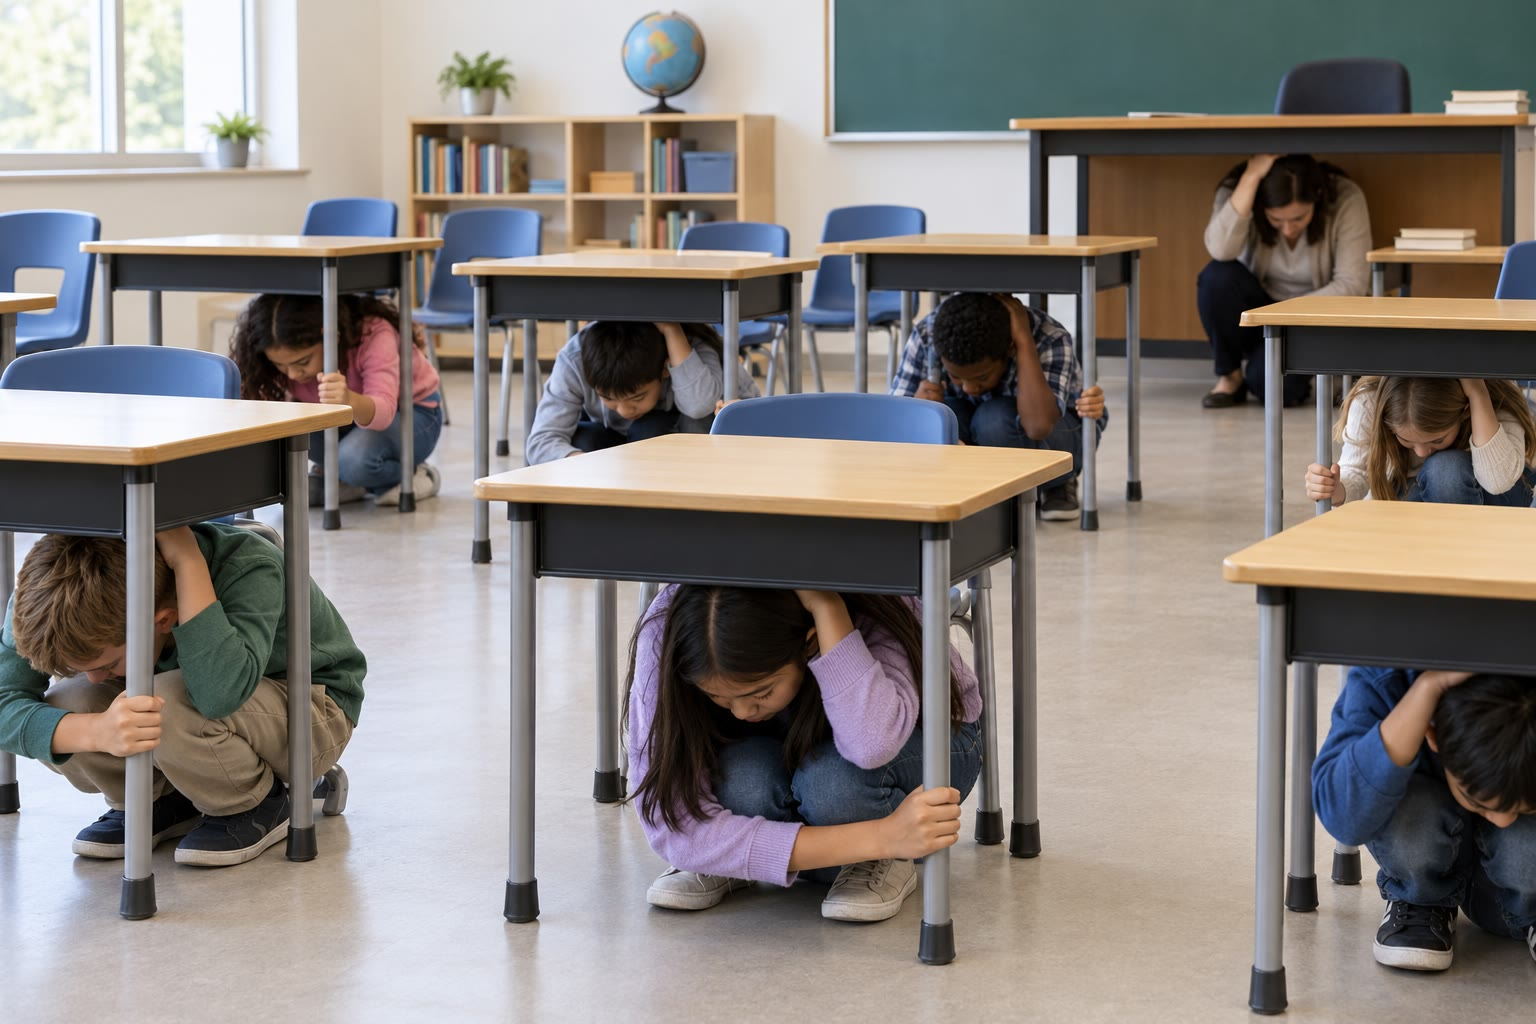
\includegraphics[width=0.55\linewidth]{images/book1/ai/g4-earthquake-drill.jpg}

{\small Un exercice d'alerte au \omterm{def:g4:volcanoes-earthquakes-first-look:earthquake}{séisme}~: les élèves s'entraînent à «~se
baisser, s'abriter et s'agripper~» sous leurs tables.}
\end{omfigure}

\section{Exercices}

\begin{exercise}[$\star$]\label{exo:g4:volcanoes-earthquakes-first-look:1}
\omterm{def:g4:volcanoes-earthquakes-first-look:eruption}{Lave}, cendres ou gaz~? (a) une \omterm{def:g1:landscapes-around-us:water}{rivière} de \omterm{def:g3:stones-pebbles-sand:rock}{roche} fondue incandescente qui
descend une pente~; (b) de minuscules morceaux de \omterm{def:g3:stones-pebbles-sand:rock}{roche} projetés dans le
ciel, qui retombent comme une \omterm{def:g4:clouds-rain-snow:precipitation}{neige} grise~; (c) quelque chose d'invisible
qui s'échappe du \omterm{def:g4:volcanoes-earthquakes-first-look:volcano}{volcan} avec les cendres.
\end{exercise}

\begin{exercise}[$\star$]\label{exo:g4:volcanoes-earthquakes-first-look:2}
Qu'est-ce qu'un \omterm{def:g4:volcanoes-earthquakes-first-look:earthquake}{séisme}~? Dure-t-il des heures, ou des secondes~?
\end{exercise}

\begin{exercise}[$\star$]\label{exo:g4:volcanoes-earthquakes-first-look:3}
Remets les trois gestes dans l'ordre~: s'agripper~; se baisser~; s'abriter.
\end{exercise}

\begin{exercise}[$\star$]\label{exo:g4:volcanoes-earthquakes-first-look:4}
Sur la \omterm{def:g2:drawing-to-map:map}{carte} de la page~\pageref{fig:g4:volcanoes-earthquakes-first-look:map},
autour de quel \omterm{def:g2:water-on-earth:ocean}{océan} se trouvent la plupart des \omterm{def:g4:volcanoes-earthquakes-first-look:volcano}{volcans}~?
\end{exercise}

\begin{exercise}[$\star$]\label{exo:g4:volcanoes-earthquakes-first-look:5}
Vrai ou faux~? (a) La plupart des \omterm{def:g4:volcanoes-earthquakes-first-look:earthquake}{séismes} sont trop faibles pour être
ressentis. (b) La \omterm{def:g4:volcanoes-earthquakes-first-look:eruption}{lave} reste liquide pour toujours. (c) Quand le sol
tremble, le plus sûr est de courir dehors.
\end{exercise}

\begin{exercise}[$\star$]\label{exo:g4:volcanoes-earthquakes-first-look:6}
Regarde le dessin du \omterm{def:g4:volcanoes-earthquakes-first-look:volcano}{volcan} de la page~\pageref{fig:g4:volcanoes-earthquakes-first-look:volcano}.
D'où vient la \omterm{def:g3:stones-pebbles-sand:rock}{roche} fondue~? Par où sort-elle~?
\end{exercise}

\begin{exercise}[$\star\star$]\label{exo:g4:volcanoes-earthquakes-first-look:7}
Sur la \omterm{def:g2:drawing-to-map:map}{carte}, trouve~: (a) un pays des Amériques qui a de nombreux \omterm{def:g4:volcanoes-earthquakes-first-look:volcano}{volcans}
sur toute sa longueur~; (b) un groupe d'îles au milieu de l'\omterm{def:g2:water-on-earth:ocean}{océan}
Pacifique, avec des \omterm{def:g4:volcanoes-earthquakes-first-look:volcano}{volcans}, qui n'est pas sur l'anneau.
\end{exercise}

\begin{exercise}[$\star\star$]\label{exo:g4:volcanoes-earthquakes-first-look:8}
Il se produit environ 141 grands \omterm{def:g4:volcanoes-earthquakes-first-look:earthquake}{séismes} par an. Environ combien cela
fait-il par mois~? (Une année a 12 mois~; donne un nombre entier.)
\end{exercise}

\begin{exercise}[$\star\star$]\label{exo:g4:volcanoes-earthquakes-first-look:9}
Environ 3 très grands \omterm{def:g4:volcanoes-earthquakes-first-look:earthquake}{séismes} sur 4 se produisent dans l'anneau autour du
Pacifique. Sur 20 très grands \omterm{def:g4:volcanoes-earthquakes-first-look:earthquake}{séismes}, environ combien t'attends-tu à en
trouver dans l'anneau~? Et en dehors~?
\end{exercise}

\begin{exercise}[$\star\star$]\label{exo:g4:volcanoes-earthquakes-first-look:10}
Pendant un exercice d'alerte au \omterm{def:g4:volcanoes-earthquakes-first-look:earthquake}{séisme}, Léo court se placer dans
l'encadrement de la porte de la classe. Qu'aurait-il dû faire à la place,
et pourquoi~?
\end{exercise}

\begin{exercise}[$\star\star\star$]\label{exo:g4:volcanoes-earthquakes-first-look:11}
Sur les 1\,214 \omterm{def:g4:volcanoes-earthquakes-first-look:volcano}{volcans} de la \omterm{def:g2:drawing-to-map:map}{carte}, 837 sont dans l'anneau autour du
Pacifique. Combien sont en dehors~? «~Environ 2 sur 3~» est-il une bonne
façon de décrire la part qui est dans l'anneau~? (Indice~: combien font
les deux tiers de 1\,200~?)
\end{exercise}
